% !TeX spellcheck = en_GB

\begin{frame}{Frequency}
	\begin{table}
		\caption{Frequencies how often the parties are mentioned.}
		\begin{tabular}{l | r | r| r|}
			Party  & Mentioned & Mentioned Bavaria & Election \\ \hline\hline
			AFD    & 11.7 \%   & 11.0 \%           & 14.6 \%  \\
			CSU    & 30.7 \%   & 32.6 \%           & 37.0 \%  \\
			FDP    & 1.9 \%    & 1.3 \%            & 3.0 \%   \\
			FW     & 47.9 \%   & 49.1 \%           & 15.8 \%  \\
			Gruene & 3.0 \%    & 1.8 \%            & 14.4 \%  \\
			Linke  & 1.3 \%    & 1.8 \%            & 1.5 \%   \\
			SPD    & 3.7 \%    & 2.1 \%            & 8.4 \%
		\end{tabular}
	\end{table}
\end{frame}

\begin{frame}{Frequency Enhanced}
	\begin{table}
		\caption{Frequencies of mentions, after Sept. 17th and most positive post per author.}
		\begin{tabular}{l | r | r| r|}
			Party  & Mentioned & Mentioned Bavaria & Election \\ \hline\hline
			AFD    & 18.7 \%   & 16.1 \%           & 14.6 \%  \\
			CSU    & 45.9 \%   & 38.1 \%           & 37.0 \%  \\
			FDP    & 1.0 \%    & n/a            & 3.0 \%   \\
			FW     & 22.0 \%   & 14.1 \%           & 15.8 \%  \\
			Gruene & 6.4 \%    & 8.1 \%            & 14.4 \%  \\
			Linke  & 1.4 \%    & 1.6 \%            & 1.5 \%   \\
			SPD    & 4.6 \%    & 4.8 \%            & 8.4 \%
		\end{tabular}
	\end{table}
\end{frame}



\begin{frame}{Timeline CSU}
	\begin{columns}
		
		\begin{column}{0.55\textwidth}
			\begin{tcolorbox}[enhanced jigsaw, colback=white, opacityback=.4, colframe=ElixirPurple, arc=3mm, boxrule=0mm, height=0.8\textheight, valign=center, title=Daily]
				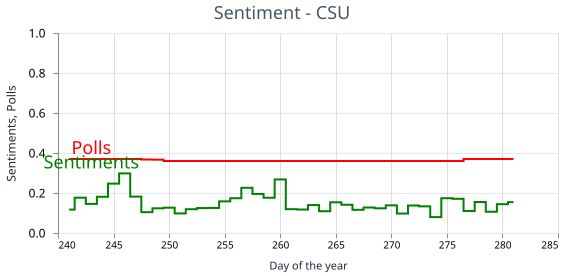
\includegraphics[width=\tcbtextwidth]{pictures/paper/comparision/visualization_csu_daily_compare.png}
			\end{tcolorbox}
		\end{column}
		
		\begin{column}{0.55\textwidth}
			\begin{tcolorbox}[enhanced jigsaw, colback=white, opacityback=.4, colframe=ElixirPurple, arc=3mm, boxrule=0mm, height=0.8\textheight, valign=center, title=Weekly]
				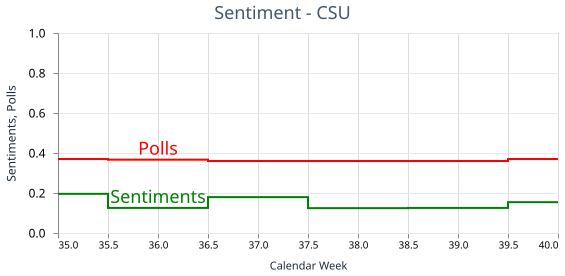
\includegraphics[width=\tcbtextwidth]{pictures/paper/comparision/visualization_csu_weekly_compare.png}
			\end{tcolorbox}
		\end{column}
	\end{columns}
\end{frame}

\begin{frame}{Timeline Freie Waehler}
	\begin{columns}
		
		\begin{column}{0.55\textwidth}
			\begin{tcolorbox}[enhanced jigsaw, colback=white, opacityback=.4, colframe=ElixirPurple, arc=3mm, boxrule=0mm, height=0.8\textheight, valign=center, title=Daily]
				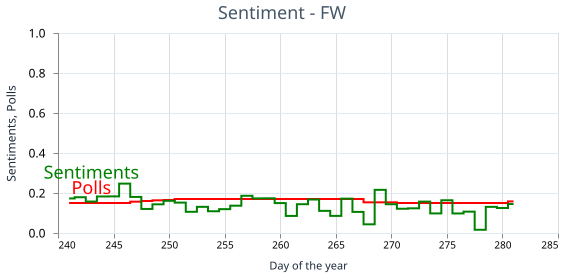
\includegraphics[width=\tcbtextwidth]{pictures/paper/comparision/visualization_fw_daily_compare.png}
			\end{tcolorbox}
		\end{column}
		
		\begin{column}{0.55\textwidth}
			\begin{tcolorbox}[enhanced jigsaw, colback=white, opacityback=.4, colframe=ElixirPurple, arc=3mm, boxrule=0mm, height=0.8\textheight, valign=center, title=Weekly]
				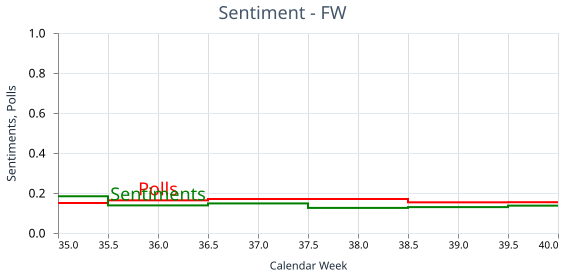
\includegraphics[width=\tcbtextwidth]{pictures/paper/comparision/visualization_fw_weekly_compare.png}
			\end{tcolorbox}
		\end{column}
	\end{columns}
\end{frame}

\begin{frame}{Sentiment vs Polls}
	\begin{figure}
		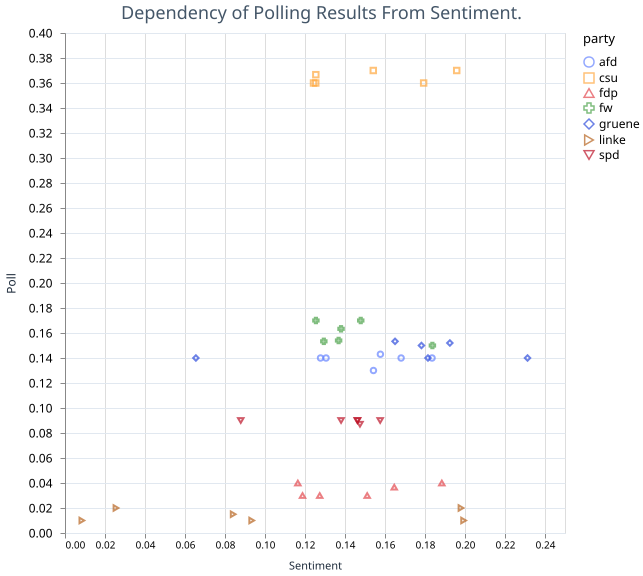
\includegraphics[width=0.5\linewidth]{pictures/paper/comparision/visualization_weekly_compare.png}
		\caption{Averaged weighted Sentiment for the parties compared to polls.}
	\end{figure}
\end{frame}
